\chapter{Analiz'a Teoretic'a}
%\pagestyle{headings}
%
\section{Introducere}
%
%\begin{center}
%\begin{figure}[h]
%    \centering
%    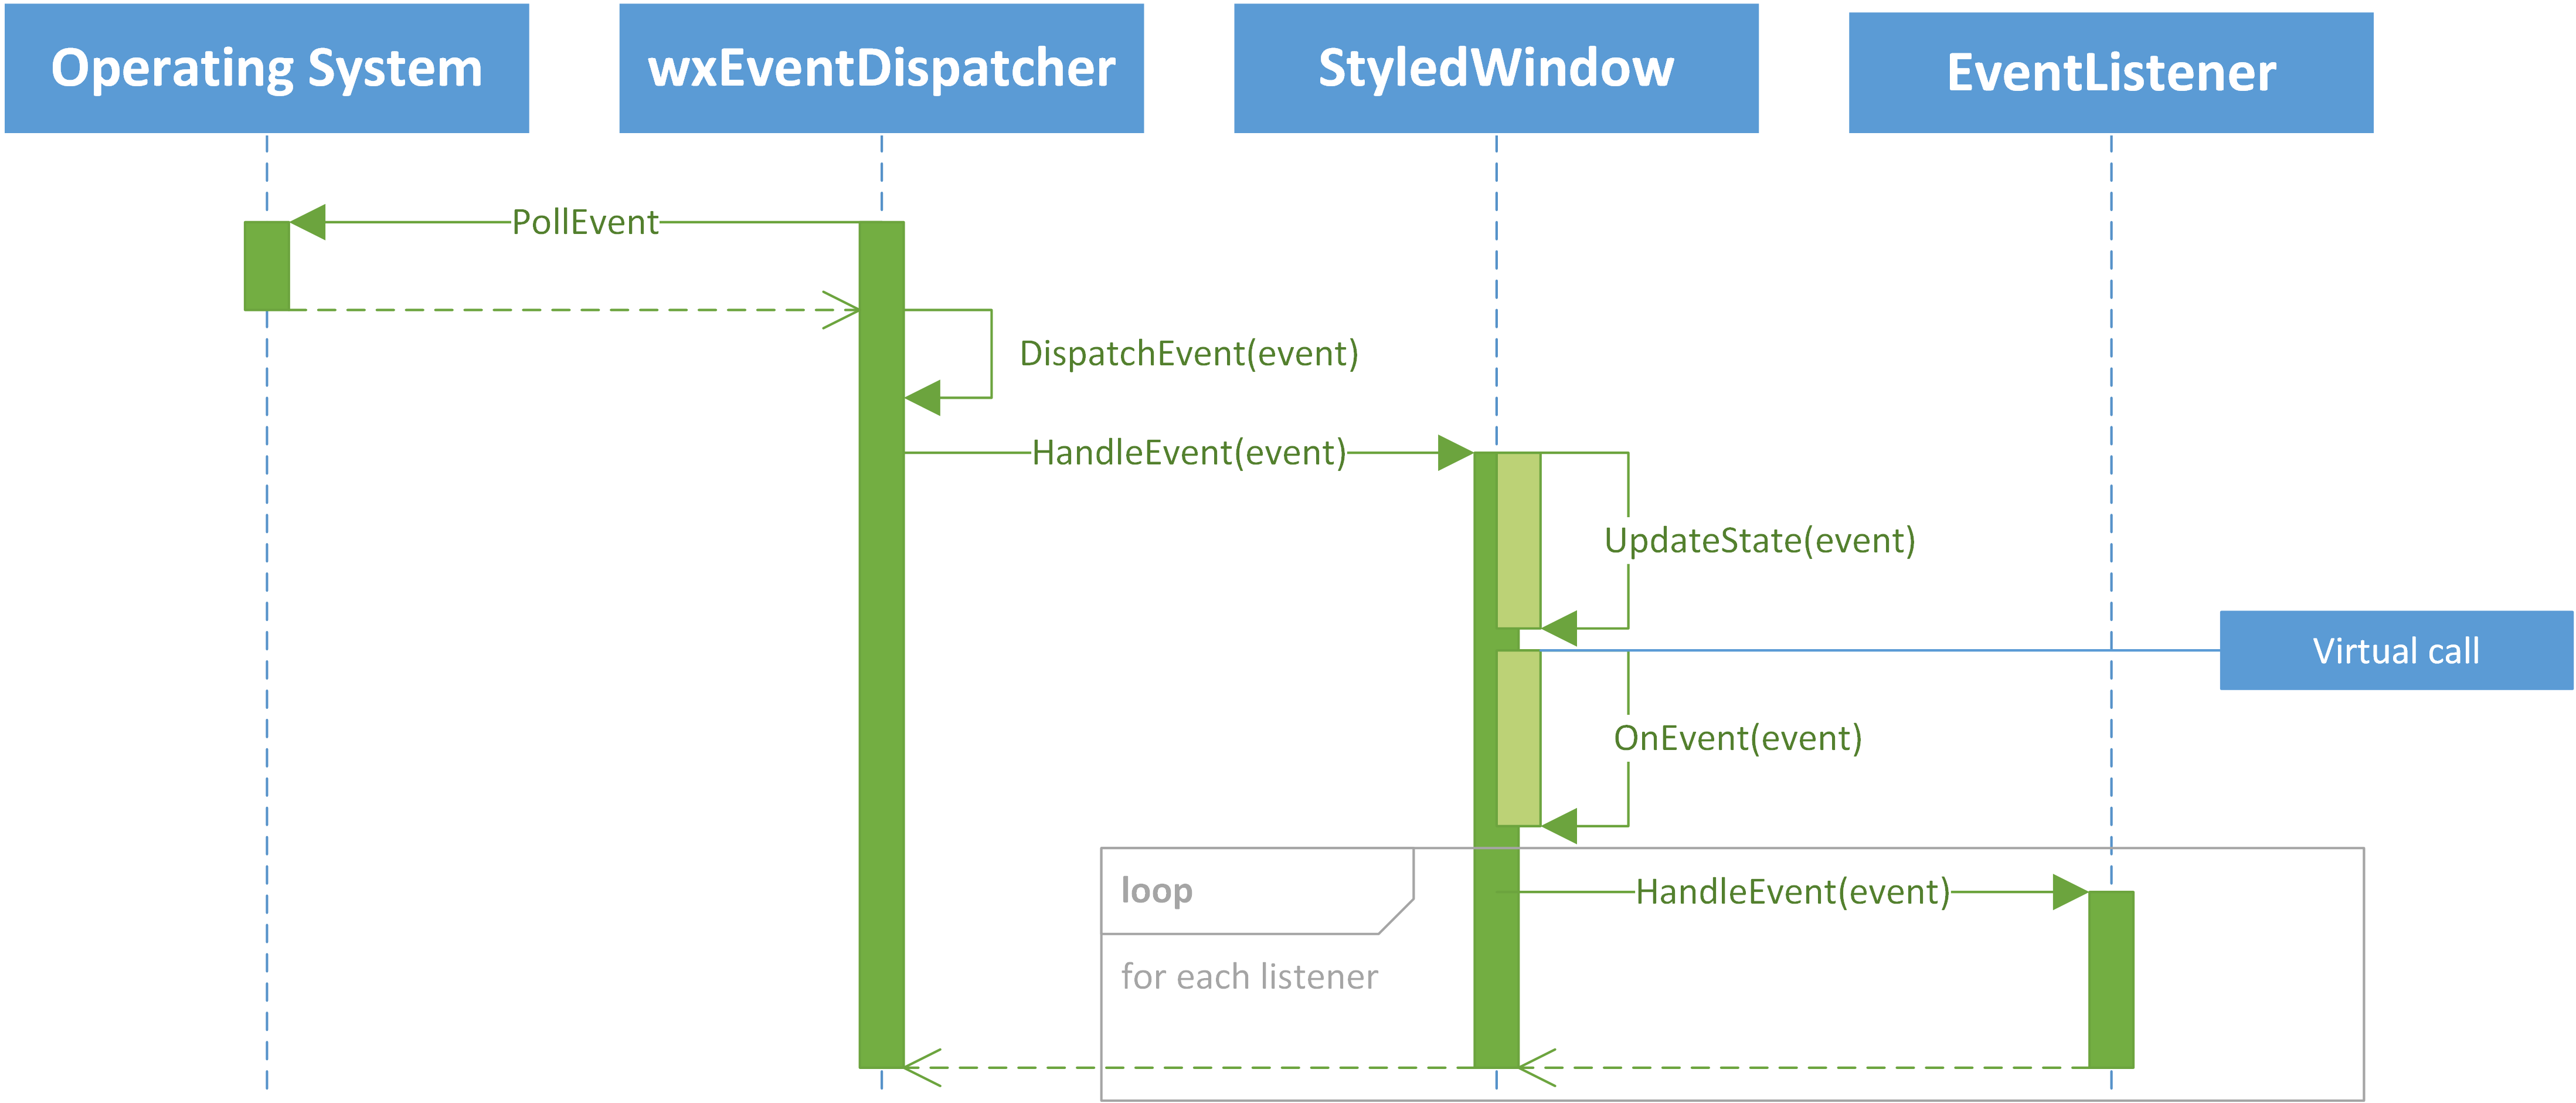
\includegraphics[scale=0.9]{img/ch4_seq_event_processing.png}
%    \label{fig0401}
%    \caption{UML Class Diagram pentru Renderer}
%\end{figure}
%\end{center}
%

Pentru a asigura o bun'a desf'a'surare a activit'a'tii de dezvoltare 'si 'intre'tinere a oric'arui proiect, pentru a asigura flexibilitate la schimb'ari 'in domeniul cerin'telor 'si pentru a preveni hazarduri ulterioare, este necesar'a o analiz'a profund'a 'si am'anun'tit'a a proiectului 'si a componentelor sale 'inainte de 'inceperea implement'arii.

\medskip

Acest capitol 

\begin{itemize}
\item {\bf Cerin'tele proiectului} sunt structurate 'in cazuri de utilizare. 'Incep{\ia}nd cu analiza cerin'telor ne asigur'am ca proiectul atinge ni'ste scopuri bine definite f'ar'a a irosi timp 'in implementarea unor tr'as'aturi nenecesare. 'In plus, putem pleca de la cerin'tele ini'tiale pentru a scrie teste 'si a valida finalizarea proiectului.
\item {\bf Analiza arhitecturilor similare} presupune suprapunerea tehnologiilor deja existente peste cerin'tele proiectului 'si a decide dac'a deciziile luate 'in dezvoltarea altor arhitecturi se aplic'a la acest proiect. 'In cazul 'in care mai multe arhitecturi diferite se prezint'a favorabile, vom decide care este mai potrivit'a.
\item {\bf Prezentarea arhitecturii finale}
\item {\bf Descrierea componentelor}
\end{itemize}

\clearpage

\section{Cazuri de utilizare}

Pentru a modela cerin'tele proiectului, prezent'am urm'atoarele cazuri de utilizare ce au rolul de a documenta cerin'tele func'tionale ale bibliotecii wxStyle.

\begin{figure}[H]
	\centering 
	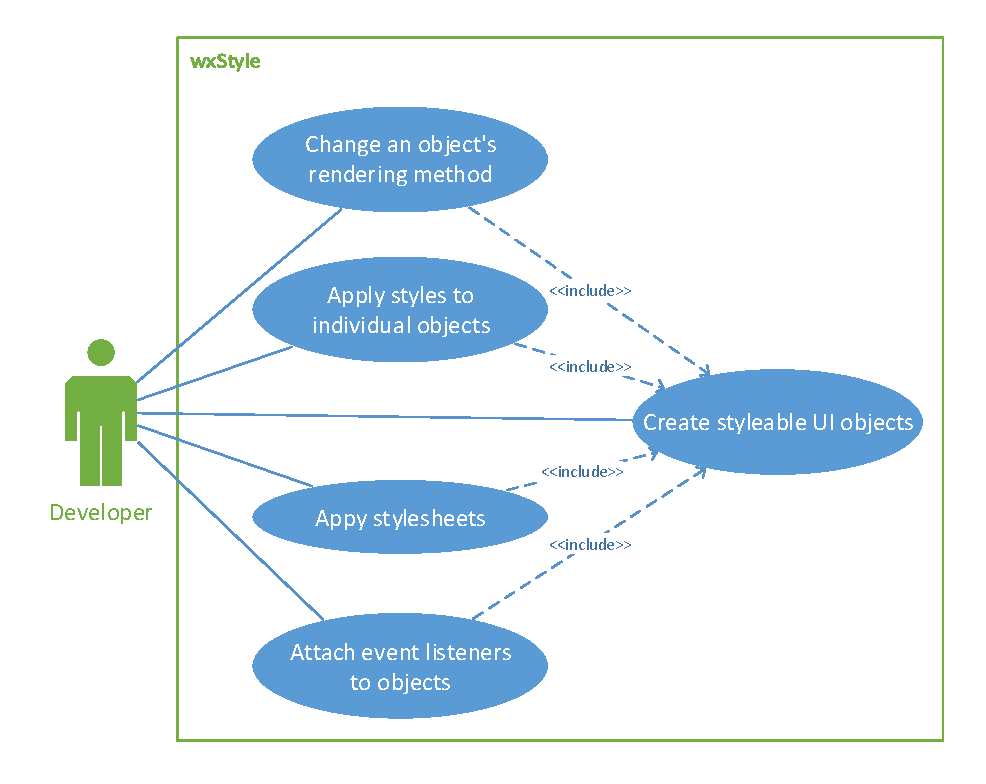
\includegraphics{img/use_case.pdf}
	\label{fig0402}
    \caption{Diagrama UML a cazurilor de utilizare}
\end{figure}

%Cazurile de utilizare prezentate 'in figura \ref{fig0402} acoper'a 

%\clearpage

\subsection{Crearea unui obiect de interfa't'a}
\textbf{Precondi'tie:} Utilizatorul a configurat un mediu de dezvoltare care are acces la bibliotecile wxWidgets 'si wxStyle.
\begin{enumerate}
\item Utilizatorul preg'ate'ste o aplica'tie vizual'a wxWidgets prin implementarea 'si instan'tierea unui wxApp.
\item Utilizatorul declar'a o variabil'a cu unul din tipurile de date ale obiectelor stilizabile 'si 'ii asigneaz'a o instan'ta a acestui tip utiliz{\ia}nd constructorul.
\item Utilizatorul amplaseaz'a obiectul de interfa't'a 'in cadrul unei ferestre, utiliz{\ia}nd constr{\ia}ngeri de amplasare, printr-un proces identic cu amplasarea obiectelor de interfa't'a implementate in biblioteca wxWidgets.
\item Utilizatorul compileaz'a 'si ruleaz'a aplica'tia.
\end{enumerate}
\textbf{Rezultat:} Obiectul de interfa't'a este prezent in cadrul ferestrei.

\subsection{Stilizarea unui obiect de interfa't'a}
\textbf{Precondi'tie:} Parcurgerea cazului de utilizare intitulat \emph{Crearea unui obiect de interfa't'a}.

\begin{enumerate}
\item Utilizatorul construie'ste o instan't'a a clasei \emph{Style} 'si apeleaz'a metodele asociate cu setarea defini'tiilor de stilizare.
\item Utilizatorul ata'seaz'a stilul la un obiect de interfa't'a stilizabil.
\item Utilizatorul compileaz'a 'si ruleaz'a aplica'tia.
\end{enumerate}
\textbf{Rezultat:} Obiectul de interfa't'a este desenat conform defini'tiilor de stil specificate 'in structura de stil.

\subsection{Modificarea procesului de prezentare al unui obiect de interfa't'a}
\textbf{Precondi'tie:} Parcurgerea cazului de utilizare intitulat \emph{Crearea unui obiect de interfa't'a}.
\begin{enumerate}
\item Utilizatorul declar'a o nou'a clasa ce implementeaz'a interfa't'a numit'a \emph{Renderer}.
\item Utilizatorul implementeaz'a metoda \emph{Draw} a acestei clase folosind primitivele de desenare oferite de wxWidgets 'si instruc'tiunile de desenare oferite de wxStyle pentru a desena o reprezentare grafic'a a obiectului de interfa't'a conform st'arii acestuia.
\item Utilizatorul ata'seaz'a o instan't'a a acestei clase unui obiect de interfa't'a stilizabil.
\item Utilizatorul compileaz'a 'si ruleaz'a aplica'tia.
\end{enumerate}
\textbf{Rezultat:} Sistemul prezin'ta obiectul de interfa't'a 'in func'tie de starea sa 'si metoda de desenare implementat'a 'in cadrul clasei de prezentare.

\subsection{Schimbarea aspectului aplica'tiei}
\textbf{Precondi'tie:} Parcurgerea cazului de utilizare intitulat \emph{Crearea unui obiect de interfa't'a}.
\begin{enumerate}
\item Utilizatorul creaz'a op'tional mai multe obiecte de interfa't'a pe care le amplaseaz'a 'in cadrul unei ferestre.
\item Utilizatorul creaz'a o structur'a \emph{Stylesheet}.
\begin{enumerate}
  \item Utilizatorul construie'ste mai multe structuri de tipul \emph{Style} cu scopul de a le asocia unui tip de obiecte de interfa't'a.
  \item Utilizatorul ata'seaz'a stilurile structurii \emph{Stylesheet} 'si le asociaz'a c{\ia}te un nume unic.
  \item Utilizatorul face asocierea dintre tipul obiectului de interfa't'a 'si stilul dorit, ambele identificate prin numele lor, utiliz{\ia}nd metodele de asociere ale structuri \emph{Stylesheet}
\end{enumerate}
\item Utilizatorul aplic'a structura \emph{Stylesheet} prin inregistrarea sa la nivel global.
\end{enumerate}
\textbf{Rezultat:} 'In urma rul'arii aplica'tiei, toate obiectele de interfa't'a stilizabile ce nu au asociate stiluri sau clase de prezentare specificate de utilizator vor fi prezentate conform stilurilor asociate tipului lor din structura \emph{Stylesheet} 'inregistrat'a la nivel global.

\subsection{Procesarea evenimentelor}
\textbf{Precondi'tie:} Parcurgerea cazului de utilizare intitulat \emph{Crearea unui obiect de interfa't'a}.
\begin{enumerate}
\item Utilizatorul identific'a sursa evenimentului, care poate fi eveniment de interac'tiune utilizator sau eveniment generat de un obiect de interfa't'a.
\item Utilizatorul declar'a o nou'a clas'a care extinde interfa't'a de tip \emph{Listener} asociat'a evenimentului.
\item Utilizatorul implementeaz'a acea metod'a care proceseaz'a evenimentul dorit.
\item Utilizatorul ata'seaz'a o instan't'a a acestei clase unuia sau mai multora obiecte de interfa't'a.
\end{enumerate}
\textbf{Rezultat:} Metoda implementa't'a de utilizator este apelat'a 'in momentul producerii unui eveniment de tipul corect.

% Motivul utilizarii
\subsection{Procesare evenimentelor}
Motivul pentru implementarea unui alt mecanism de procesare al evenimentelor este de a oferi posibilitatea mai multor obiecte sa raspunda la evenimente. In momentul in care o rutina de procesare al evenimentului este legat'a de un anumit tip de eveniment si un anumit obiect, evenimentele de acel tip produse de acel obiect nu vor mai putea fi procesate de alta rutin'a. Acest lucru ingreuneaz'a biblioteca wxStyle, deoarece obiecte precum ResizeHandler 'si DragHandler trebuie sa poata intercepta evenimentele produse de dispozitiv-ul mouse f'ar'a a intrerupe propagarea acestora c'atre obiectul c'arora le este destinat. Dac'a aceste evenimente nu ar ajunge la obiectul destinatar, acesta nu ar putea s'a-'si actualizeze starea sau s'a genereze evenimente abstracte specifice obiectului precum ap'asarea unui buton sau mutarea indicatorului de text 'in interiorul unui obiect de interfa't'a pentru introducerea de text.

Cel mai popular mecanism de distribuire a unui eveniment este cel bazat pe sablonul Observer. Acest mecanism presupune prezen'ta a dou'a componente: un produc'ator de evenimente 'si mai mul'ti 'ascult'atori de evenimente. Ascult'atorii se pot 'inregistra la produc'ator pentru a fi notifica'ti 'in cazul 'in care un nou eveniment este produs. La orice moment, un ascult'ator se poate deinregistra de la produc'ator. Produc'ator men'tine o list'a de ascult'atori. Ac'tiunile de inregistrare si deinregistrare se traduc 'in ac'tiuni de manipulare a listei precum ad'augarea unui noi observator sau 'stergerea unuia deja existent. Notificarea observatorilor presupune apelarea unei metode a obiectului observator. Aceste metode sunt predefinite de interfa't'a observatorului. Fiecare produc'ator accept'a doar un anumit tip de observator, pentru a asigura prezen'ta metodelor de procesare. 'In momentul gener'arii unui nou eveniment, produc'atorul notific'a toti observatorii. Utiliz{\ia}nd acest mecanism, putem procesa acela'si eveniment din locuri multiple.

O problem'a la mecanismul de observator pentru procesarea evenimentelor este ordinea 'in care observatorii sunt notifica'ti de prezent'a unui eveniment. Dorim s'a ne asigur'am c'a obiectele de interfa't'a c'arora le este destinat evenimentul au ocazia s'a 'il proceseze 'inaintea altor observatori inregistrati de c'atre utilizatori. Din acest motiv, evenimentele sunt procesate 'in trei etape:

1. Clasa StyledWindow primeste evenimentul de la biblioteca wxStyle prin mecanismul standard wxWidgets. In cadrul acestei rutine, StyledWindow adjusteaz'a starea obiectului precum: dac'a este sau nu ap'asat, daca dispozitivul mouse se afl'a sau nu deasupra obiectului, etc.
2. StyledWindow apeleaza metoda virtuala On{Event} care este implementat'a (la nevoie) de tipul real al obiectului. In acest fel, obiectele de interfa't'a au ocazia s'a interpreteze evenimentele pentru a-'si 'intre'tine propria stare intern'a.
3. StyledWindow notific'a to'ti observatorii inregistra'ti pentru evenimentul respectiv. Ordinea 'in care ace'stia sunt notifica'ti este aceea 'in care ei s-au 'inregistrat.

Deoarece clasa StyledWindow are responsabilitatea de a 'intre'tine starea obiectului, de a apela metoda virtual'a de procesare 'si de a notifica to'ti observatorii asigur'a corectitudinea proces'arii evenimentelor. Obiectele specifice de interfa't'a nu au responsabilitatea de a 'intre'tine o list'a de observatori sau de a procesa evenimentele 'intr-o anumit'a ordine.

% Rough Ideas
\subsection{Stilul implicit}
Pentru a putea utiliza u'sor 'si sigur mecanismul de stilizare, avem nevoie de garan'tia c'a defini'tiile obligatorii ale unui stil exist'a. Defini'tiile obligatorii sunt acele defini'tii f'ar'a de care nu se poate construi o reprezentare a obiectului de interfa't'a. De exemplu: defini'tiile pentru font, culoarea planului prioritar (foreground), combina'tia de defini'tii care descriu opacitatea 'si modul de prezentare al fundalului. Aceste defini'tii, dac'a nu sunt explicit setate, trebuie s'a aibe o valoare predefinit'a. Aceast'a valoare predefinit'a provine de la stilul implicit al bibliotecii wxStyle. Prin mecanismul de mo'stenire al stilurilor, toate defini'tiile setate manual de utilizator se vor aplica deasupra stilului implicit. Stilul implicit este urm'atorul:

% BLA, BLA, BLA

De asemenea, mecanismul de stilizare prin fi'siere de stil \emph{stylesheets} trebuie sa poata stiliza 'intreaga aplica'tie la orice moment 'in timpul rul'arii acesteia. Acest lucru presupune modificarea tuturor obiectelor de interfata ce nu au stiluri sau proceduri de prezentare predefinite din componen'ta aplica'tiei. Implementarea acestui mecanism poate fi facut'a 'in dou'a moduri:

1. Prin men'tinerea unei liste de obiecte vizuale care s'a con'tin'a toat'e obiectele de interfa't'a din componen'ta aplica'tiei. La momentul stiliz'arii aplica'tiei, toate obiectele din list'a vor fi parcurse, iar stilurile sau metodele lor de prezentare vor fi actualizate.
2. Prin men'tinerea unei liste de stiluri implicite, indexate dup'a tipul obiectului de interfa't'a c'aruia 'ii sunt asociate. Schimbarea stilului aplica'tiei implic'a updatarea stilulurilor din aceast'a lista. La momentul prezent'arii unui obiect ce nu are un stil sau un obiect de prezentare definit de utilizator, acesta interogheaz'a lista de stiluri 'si obiecte de prezentare standard.

Metoda num'arul 1 implic'a stocarea 'in memorie a tuturor instan'telor de obiecte vizuale din aplica'tie, 'intr-o structur'a de date de tip list'a. Aceast'a list'a este greu de 'intre'tinut deoarece obiectele trebuiesc 'sterse din list'a 'in momentul 'in care acestea sunt distruse. Mai mult, modificarea unui stil predefinit implic'a parcurgerea 'intregii liste, indiferent dac'a obiectul este vizibil sau nu. Totu'si, lista va fi parcurs'a o singur'a dat'a pentru fiecare schimbare 'in setul de stiluri predefinite ale aplica'tiei. De cele mai multe ori, acest lucru se va realiza de doua ori: prima data pentru setarea stilului implicit al bibliotecii, iar a doua oara pentru setarea stilurilor specificate implicit de c'atre utilizator. Pentru a nu suprapune stilul implicit peste un stil setat de utilizator, toate obiecte de interfa't'a vor trebui augmentate cu un membru boolean care s'a indice dac'a stilul sau obiectul de prezentare al obiectului de interfa't'a este sau nu setat explicit de c'atre utilizator.

Metoda num'arul 2 are avantajul c'a nu necesit'a men'tinerea unei structuri de date suplimentare pentru stocarea instan'telor obiectelor de interfa't'a. 'In schimb, aceast'a metoda presupune stocarea stilurilor, 'si delegarea opera'tiei de citire a stilurilor c'atre fiecare obiect de interfa't'a. In mod similar primei metode, aceast'a metod'a necesit'a augmentarea cu membrul suplimentar care s'a disting'a dintre stiluri si obiecte de prezentare setate de utilizator, si cele implicite. Doar obiectele ce nu au stiluri setate explicit vor apela la cele implicite. Accesul la stilurile si obiectele de interfa't'a implicite se poate face printr-o instan'ta global'a 'si unic'a a unei clase ce are singurul rol de a stoca aceast'a informa'tie. O alt'a metod'a este de a oferi tuturor obiectelor de interfa't'a o instan'ta a unei clase ce poate "produce" stiluri si obiecte de prezentare specializate pentru tipul obiectului de interfa't'a. Folosim verbul "produce", deoarece dorim ca instantele de stiluri sa poat'a varia 'in timpul rul'arii, deci nu putem trimite instan'te concrete. Mai degrab'a trimitem un obiect care poate construi instan'te variabile 'in timpul rul'arii.




%\section{Design patterns}
%
%\subsection{Observer}
%
%\subsection{Singleton}
%
%\subsection{Factory}
